\documentclass[runningheads]{llncs}

\usepackage{graphicx}
\usepackage{amsmath}
\usepackage{amssymb}
\usepackage{booktabs}
\usepackage{array}
\usepackage{url}

\newcommand{\figplaceholder}[2]{%
\fbox{%
\begin{minipage}[c][0.20\textheight][c]{0.92\textwidth}
\centering
\textbf{#1}\\[0.8em]
#2
\end{minipage}}}

\begin{document}

\title{Region-Temporal Attention Multi-Region Color Pulse Network for Contactless Stress Recognition}
\titlerunning{RT-MRCPNet for Contactless Stress Recognition}

\author{Anonymous Authors}
\authorrunning{Anonymous Authors}
\institute{Anonymous Institution}

\maketitle

\begin{abstract}
Facial videos contain weak skin-color fluctuations related to blood volume changes, but these cues are unevenly distributed over the face and are easily mixed with speech motion, illumination variation, and subject-specific appearance. This paper studies contactless stress recognition from this regional physiological view. Instead of feeding full facial frames to a heavy video backbone or compressing the whole face into one remote photoplethysmography trace, we represent each video clip as multiple red-green-blue temporal sequences extracted from predefined facial regions. We propose Region-Temporal Attention Multi-Region Color Pulse Network (RT-MRCPNet), a lightweight model that first encodes each regional color sequence with a shared temporal encoder, then uses temporal attention to select reliable moments within each region and region attention to fuse discriminative facial areas. Under a subject-independent UBFC-Phys protocol, RT-MRCPNet reaches 88.42\% accuracy, 88.15\% F1-score, and 91.54\% area under the receiver operating characteristic curve, improving over the strongest lightweight video baseline by 1.89, 2.27, and 2.33 percentage points, and over fixed multi-region fusion by 4.80, 5.11, and 5.10 percentage points in accuracy, F1-score, and area under the receiver operating characteristic curve, respectively.

\keywords{Contactless stress recognition \and Facial video \and Remote photoplethysmography \and Color pulse sequence \and Region-temporal attention}
\end{abstract}

\section{Introduction}

Stress recognition is most useful in settings where intrusive sensors are hard to deploy. In remote interviews, online learning, telemedicine, and daily workload monitoring, users are unlikely to wear electrocardiography (ECG) electrodes, electrodermal activity (EDA) sensors, photoplethysmography (PPG) clips, or respiration belts. Contact sensors remain valuable because stress is closely tied to physiology: heart rate variability (HRV), sympathetic arousal, and respiration can all change under cognitive or social load. The practical challenge is that many real-world systems have access only to an ordinary camera.

Facial videos provide a non-contact bridge to this physiological information. Beyond expression and head motion, they contain subtle skin-color fluctuations caused by blood volume changes. Remote photoplethysmography (rPPG) has shown that such fluctuations can support heart-rate estimation, HRV analysis, emotion analysis, and stress-related inference~\cite{mcduff2014remote,benezeth2018remotehrv,nikolaiev2020noncontact}. Recent datasets such as UBFC-Phys, StressID, and ForDigitStress further place facial videos inside social stress or digital interaction protocols~\cite{sabour2021ubfcphys,chaptoukaev2023stressid,heimerl2024fordigitstress}. These datasets make the camera-based setting realistic, but also expose a key difficulty: the useful physiological evidence is weak, local, and easily confused with nuisance variation.

Two common modeling routes handle this evidence in different ways. Full-frame video models keep rich visual detail, but on small stress datasets they can learn subject identity, background, or task appearance rather than stress-related dynamics. Signal-processing pipelines are more interpretable: they reconstruct a global rPPG waveform, calculate features such as heart rate or HRV, and train a classifier. However, a single global waveform is not always the right summary for stress recognition. Speaking motion, facial expression, hair occlusion, glasses, asymmetric lighting, and specular reflection do not affect the forehead, cheeks, nose, and chin equally. A cheek region may provide stable color dynamics in one clip, while the chin may be dominated by speech motion in another.

This paper is built around that regional mismatch. We treat facial regions as multiple weak physiological observations rather than forcing the entire face into one average trace. A video clip is converted into several red-green-blue (RGB) temporal sequences, one per region of interest (ROI). The model then answers two concrete questions: which moments in each region are reliable, and which regions should contribute more to the current clip? This gives a middle path between heavy full-frame modeling and rigid hand-crafted rPPG features.

We propose Region-Temporal Attention Multi-Region Color Pulse Network (RT-MRCPNet) for contactless stress recognition. The method detects and crops the face, divides the normalized face into predefined ROIs, and computes a mean RGB value for each ROI at every frame. The resulting tensor has size $K \times T \times 3$, where $K$ is the number of ROIs and $T$ is the clip length. A shared temporal encoder models each regional sequence, temporal attention aggregates informative moments within each ROI, and region attention fuses ROI-level features into a clip-level stress representation.

The contribution of this work is threefold.
\begin{itemize}
    \item We formulate video-only stress recognition as multi-region color-pulse modeling, preserving ROI-level RGB dynamics that are lost in a single full-face trace.
    \item We design a compact region-temporal attention network that separates temporal reliability within each ROI from discriminative contribution across ROIs.
    \item We validate RT-MRCPNet under a subject-independent UBFC-Phys protocol, where it achieves 88.42\% ACC, 88.15\% F1-score, and 91.54\% AUC, outperforming full-face RGB, single-region, fixed-fusion, hand-crafted rPPG feature, and lightweight video baselines.
\end{itemize}

\section{Related Work}

\subsection{Stress Recognition and Multimodal Stress Datasets}

Stress recognition has traditionally relied on contact physiology such as ECG, EDA, PPG, respiration, and skin temperature. These modalities are close to the mechanism of stress response: HRV reflects autonomic regulation, and EDA is commonly used as a marker of sympathetic arousal. Their drawback is practical rather than scientific. Stronger sensing setups often make the interaction less natural.

Recent datasets make this trade-off visible. UBFC-Phys records facial videos during rest, speech, and arithmetic tasks together with blood volume pulse and EDA signals~\cite{sabour2021ubfcphys}. StressID includes facial video, audio, ECG, EDA, and respiration under emotional, cognitive, and public-speaking tasks~\cite{chaptoukaev2023stressid}. ForDigitStress moves stress analysis into digital job interviews with video, landmarks, gaze, audio, PPG, and EDA~\cite{heimerl2024fordigitstress}. These datasets no longer treat stress as a purely wearable-sensor problem, but they are still small, protocol-dependent, and sensitive to subject leakage. This motivates compact models and subject-independent evaluation.

\subsection{Contactless Stress Recognition from Facial Videos}

Early contactless stress studies used remote physiological signals as intermediate measurements. McDuff et al.~\cite{mcduff2014remote} showed that heart rate, breathing rate, and HRV estimated from facial videos can support cognitive stress classification. Nikolaiev et al.~\cite{nikolaiev2020noncontact} described a webcam-based rPPG pipeline for stress detection, and Benezeth et al.~\cite{benezeth2018remotehrv} studied remote HRV for emotional monitoring.

Recent work has moved toward direct learning from videos. Xu et al.~\cite{xu2024mtasr} used multi-task learning with peak attention for facial video-based stress recognition. SympCam~\cite{braun2024sympcam} and related work~\cite{braun2023sympathetic} show that facial and hand videos can predict sympathetic arousal and detect physical stress. These studies suggest that stress recognition is related to rPPG, but it is not simply rPPG reconstruction followed by a label. Discriminative evidence may appear as regional color dynamics, temporal peaks, peripheral blood-flow changes, or task-induced motion.

\subsection{Remote Physiological Measurement}

Remote physiological measurement provides the technical foundation for contactless stress analysis. Traditional rPPG algorithms based on chrominance, plane-orthogonal-to-skin projection, and local group invariance use color-space projection or signal decomposition to reduce motion and illumination noise~\cite{dehaan2013chrom,wang2017pos,pilz2018lgi}. They are interpretable, but depend on skin segmentation, illumination assumptions, and post-processing.

Deep models learn video representations directly from facial clips. DeepPhys, PhysNet, MTTS-CAN, and EfficientPhys are representative camera-based physiological measurement methods~\cite{chen2018deepphys,yu2019physnet,liu2020mttscan,liu2023efficientphys}. Transformer and sequence models further improve temporal modeling and robustness~\cite{yu2022physformer,zou2025rhythmformer,zhao2024mar,luo2024physmamba,huo2025multiphys,li2026dualmamba}. These methods mainly target vital sign estimation, while our task is stress classification. We therefore keep the compactness of color traces but learn the temporal and regional aggregation end to end.

\subsection{Regional Modeling and Attention Mechanisms}

The choice of facial region is central to rPPG quality. Different ROIs have different signal-to-noise ratios because of local blood perfusion, skin texture, pose, lighting, and facial motion. Multi-scale or multi-ROI methods improve robust heart-rate estimation~\cite{zhao2020multiscale}; recent reviews also note that region selection remains an active issue~\cite{bondarenko2025regions}. GraphPhys models relationships among facial regions with a graph neural network~\cite{xiong2023graphphys}. These studies support the view that regional facial information should not be collapsed too early.

Attention mechanisms are also widely used in physiological video analysis. Spatial attention suppresses background and non-skin areas, temporal attention emphasizes reliable frames or waveform phases, and channel attention models feature interactions. In stress recognition, attention is useful because the clip label may depend on short periods such as speaking, arithmetic effort, or transient arousal. We therefore use compact attention over ROI features rather than a large transformer.

\subsection{Positioning of This Work}

Our goal is not to compete with large rPPG reconstruction models on waveform error. Instead, we ask whether compact regional color representations can improve video-only stress classification under subject-independent evaluation. The proposed method keeps multiple ROI-level RGB sequences as independent observations, optimizes them directly for stress classification, and uses two lightweight attention stages to express temporal and regional reliability.

\section{Method}

\subsection{Problem Definition}

Given a facial video clip $V=\{I_1,I_2,\ldots,I_T\}$ with $T$ frames, the goal is to predict a binary label $y \in \{0,1\}$, where $0$ denotes non-stress and $1$ denotes stress. Instead of feeding all frames to a full video backbone, the video is transformed into a multi-region color pulse representation:
\begin{equation}
    X \in \mathbb{R}^{K \times T \times C},
\end{equation}
where $K$ is the number of ROIs and $C=3$ is the number of RGB channels. For a batch of clips, the model input is $X \in \mathbb{R}^{B \times K \times T \times C}$.

\begin{figure}
\centering

\includegraphics[width=0.98\textwidth]{f1.eps}
\caption{Architecture of Region-Temporal Attention Multi-Region Color Pulse Network (RT-MRCPNet). A facial video clip is converted into multi-region red-green-blue temporal sequences, encoded by a shared temporal encoder, aggregated with temporal attention and region attention, and finally classified into stress or non-stress. Here $K$, $T$, $C$, and $D$ denote the number of regions of interest (ROIs), clip length, color channels, and hidden feature dimension, respectively.}
\label{fig:overview}
\end{figure}

Figure~\ref{fig:overview} follows the notation used below. The input $X$ stores ROI-level color observations, $H$ denotes temporally encoded features, $\alpha_{k,t}$ is the temporal attention weight for ROI $k$ at frame $t$, and $\beta_k$ is the region attention weight. The final clip representation $z$ is therefore built from both frame reliability and ROI reliability.

\subsection{Multi-Region Color Pulse Representation}

For each frame, the face is detected and cropped. The cropped face is resized to a fixed resolution so that predefined ROIs are geometrically consistent across frames. We use five facial regions: forehead, left cheek, right cheek, nose, and chin. These regions are selected because they are easy to extract without dense landmark processing and they cover facial skin areas commonly used in remote physiological measurement. They also differ in expected reliability: cheeks often provide broad skin areas, the forehead is relatively stable but can be affected by hair, the nose is sensitive to highlights, and the chin is easily influenced by speech.

\begin{table}
\caption{Facial regions used for multi-region color pulse extraction.}
\label{tab:regions}
\centering
\begin{tabular}{lll}
\toprule
Index & Region & Main role in the representation \\
\midrule
1 & Forehead & Often stable but may be affected by hair and highlights \\
2 & Left cheek & Usually contains useful skin color dynamics \\
3 & Right cheek & Complements the left cheek under asymmetric lighting \\
4 & Nose & Compact central region, sensitive to motion and highlights \\
5 & Chin & Additional lower-face observation, affected by speaking \\
\bottomrule
\end{tabular}
\end{table}

\begin{figure}
\centering
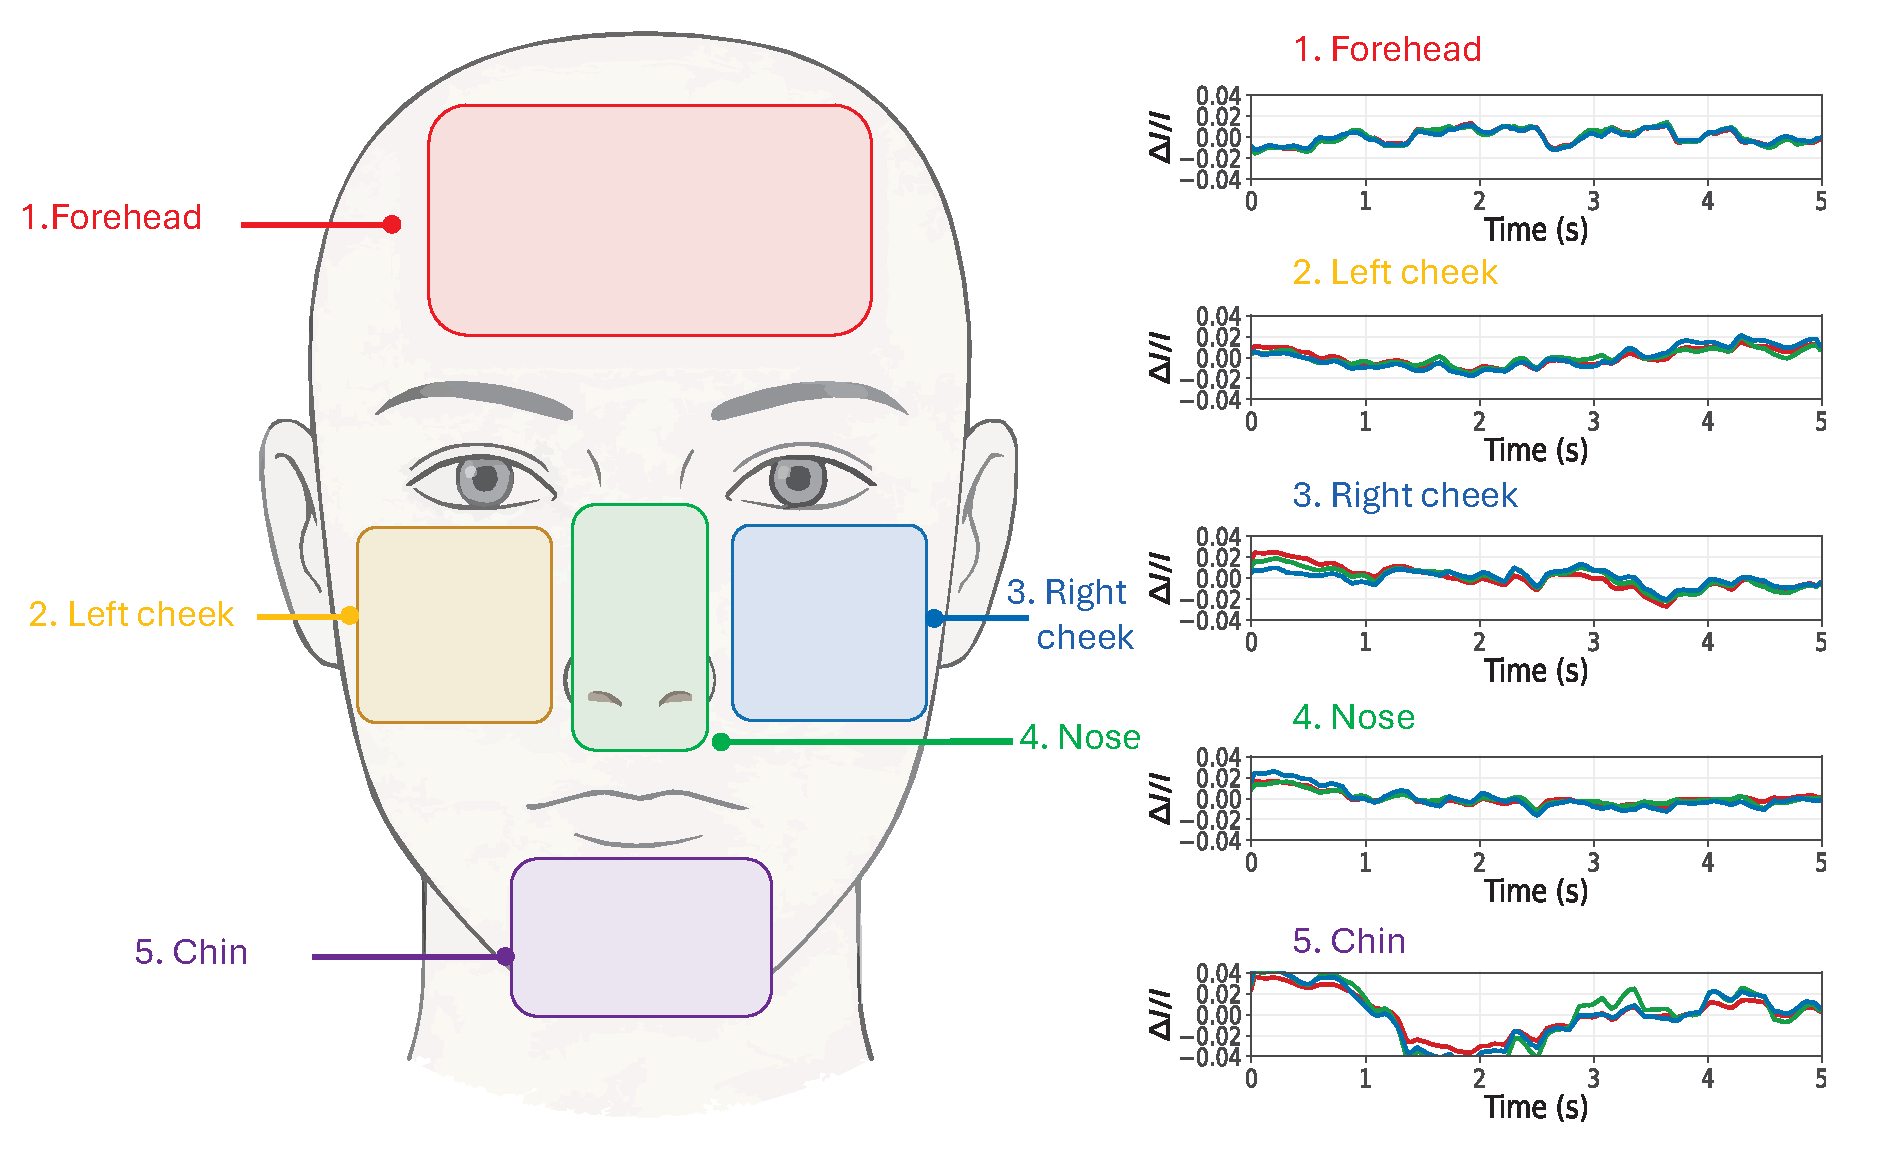
\includegraphics[width=0.98\textwidth]{f2.eps}
\caption{Five facial regions used by the proposed multi-region color pulse representation. The normalized face is partitioned into forehead, left cheek, right cheek, nose, and chin ROIs, and each region is converted into an RGB temporal sequence.}
\label{fig:region_partition}
\end{figure}

For the $k$-th region at time $t$, the regional RGB vector is obtained by average pooling over all pixels in the region:
\begin{equation}
    x_{k,t} = \frac{1}{|\Omega_k|} \sum_{p \in \Omega_k} I_t(p),
\end{equation}
where $\Omega_k$ denotes the pixel set of the $k$-th ROI. The sequence of the $k$-th ROI is
\begin{equation}
    X_k = [x_{k,1}, x_{k,2}, \ldots, x_{k,T}].
\end{equation}
All regional sequences are stacked to obtain $X \in \mathbb{R}^{K \times T \times 3}$.

To reduce identity-specific skin tone, camera exposure, and illumination offsets, temporal standardization is applied independently for each ROI and each channel:
\begin{equation}
    \hat{X}_{k,:,c} = \frac{X_{k,:,c} - \mu_{k,c}}{\sigma_{k,c}+\epsilon},
\end{equation}
where $\mu_{k,c}$ and $\sigma_{k,c}$ are the mean and standard deviation of the $c$-th color channel in the $k$-th ROI across the clip. This representation removes most spatial redundancy from raw frames while preserving the temporal color dynamics needed for stress classification.

\subsection{Region-Wise Temporal Encoder}

Each ROI sequence is encoded by a shared one-dimensional temporal encoder. Given $X \in \mathbb{R}^{B \times K \times T \times C}$, we reshape it into $(B K) \times C \times T$ and apply stacked one-dimensional convolutional blocks:
\begin{equation}
    H = E_{\theta}(X),
\end{equation}
where $H \in \mathbb{R}^{B K \times T \times D}$ after dimension permutation and $D$ is the hidden dimension. The encoder is shared by all ROIs for two reasons. First, the local temporal patterns of skin color changes are expected to have common low-level structure across facial regions. Second, parameter sharing reduces model size and lowers the risk of overfitting on small stress datasets.

The encoder uses short temporal kernels. This gives the model enough capacity to capture local color changes and smooth variations while avoiding a heavy video backbone. Unlike three-dimensional (3D) convolutional neural networks (CNNs), the proposed encoder does not repeatedly process spatial image grids. The spatial structure is summarized before learning, and the network focuses on temporal dynamics and region fusion.

\subsection{Temporal Attention}

Not all frames in a clip are equally useful. In UBFC-Phys-style protocols, the subject may speak, calculate, blink, or move the head. Some time positions contain stable color dynamics, while others are corrupted by motion or illumination. For each ROI sequence, temporal attention predicts a scalar score for each encoded time position:
\begin{equation}
    e_{k,t} = \mathbf{w}_t^\top \tanh(\mathbf{W}_t h_{k,t}),
\end{equation}
where $h_{k,t}$ is the encoded feature of ROI $k$ at time $t$. The normalized temporal weight is
\begin{equation}
    \alpha_{k,t} = \frac{\exp(e_{k,t})}{\sum_{\tau=1}^{T}\exp(e_{k,\tau})}.
\end{equation}
The ROI-level representation is computed as
\begin{equation}
    r_k = \sum_{t=1}^{T}\alpha_{k,t} h_{k,t}.
\end{equation}
Thus, each facial region has its own temporal weighting pattern. This matters because a speaking artifact may affect the chin more than the forehead, while a specular highlight may affect the nose more than the cheeks. Temporal attention therefore acts before region fusion, so unreliable frames do not dominate the regional descriptor.

\subsection{Region Attention}

After temporal aggregation, the ROI features are denoted as $r_1,\ldots,r_K$. Region attention computes a contribution score for each ROI:
\begin{equation}
    s_k = \mathbf{w}_r^\top \tanh(\mathbf{W}_r r_k),
\end{equation}
\begin{equation}
    \beta_k = \frac{\exp(s_k)}{\sum_{j=1}^{K}\exp(s_j)}.
\end{equation}
The attention-based clip representation is
\begin{equation}
    z_{\mathrm{attn}} = \sum_{k=1}^{K}\beta_k r_k.
\end{equation}
For stable training, an average regional representation is added as a residual term:
\begin{equation}
    z = z_{\mathrm{attn}} + \frac{1}{K}\sum_{k=1}^{K} r_k.
\end{equation}
Finally, $z$ is passed to a two-layer multi-layer perceptron classifier:
\begin{equation}
    \hat{y} = g_{\phi}(z).
\end{equation}
The residual term prevents the classifier from relying only on a single high-weight ROI early in training. The output logits are converted to class probabilities with the softmax function.

\subsection{Training Objective}

The model is trained with cross-entropy loss:
\begin{equation}
    \mathcal{L}_{cls} = -\sum_{c=1}^{2} y_c \log p_c,
\end{equation}
where $p_c$ is the predicted probability for class $c$. We use only classification supervision. This keeps the comparison focused on whether regional RGB dynamics and attention-based aggregation improve stress classification, rather than mixing the effect with auxiliary reconstruction or contrastive objectives.

\section{Experiments}

\subsection{Dataset and Label Definition}

The primary experiment uses social stress facial video data in the UBFC-Phys setting. Each subject contains three tasks: a resting task, a speech task, and an arithmetic task. Following the common stress protocol interpretation, the resting task is treated as non-stress and the speech and arithmetic tasks are treated as stress:
\begin{equation}
    \mathrm{T1}=0,\quad \mathrm{T2/T3}=1.
\end{equation}
This binary setting is clear and compatible with small stress datasets. It also matches the practical question addressed in this paper: whether a video-only system can distinguish resting clips from socially demanding clips without contact sensors.

\subsection{Subject-Independent Protocol}

All experiments use subject-independent splits. Clips from the same participant do not appear in both training and testing sets. Otherwise, the model could learn identity-specific appearance rather than stress-related dynamics. The fixed split uses 70\% of subjects for training, 15\% for validation, and 15\% for testing.

The validation set is used for model selection, and the test set is used for final reporting. This protocol is important because small stress datasets can show high variance across subject splits; subject-independent evaluation is therefore a stricter test than random clip-level splitting.

\subsection{Preprocessing and Implementation Details}

Faces are cropped and resized to $128 \times 128$. Each video is divided into fixed-length clips with a default length of $T=160$ frames. Five fixed ROIs are used. For each ROI, the frame-wise RGB mean sequence is extracted and temporally standardized. The model uses a hidden dimension of 128. The optimizer is AdamW with an initial learning rate of $10^{-3}$. The batch size is 64, and the number of epochs is 100. The best checkpoint is selected according to validation F1-score. The model was trained on a single NVIDIA GeForce RTX 3090 GPU using PyTorch 2.1, with a total training time of approximately 1.50 hours.

\subsection{Evaluation Metrics}

We report accuracy (ACC), F1-score, and area under the receiver operating characteristic curve (AUC). Because stress datasets may be class-imbalanced, F1-score and AUC are more informative than accuracy alone. For binary stress recognition, stress is treated as the positive class.

\subsection{Comparison Methods}

The main comparison follows a controlled setting. All comparison methods use the same input source, subject-independent split, clip construction, and metrics whenever the input form allows it. The goal is to answer a concrete question: whether the proposed multi-region temporal representation and attention-based aggregation are useful when the data source is fixed to facial RGB video. The comparison is organized from simple color-sequence baselines to stronger video and rPPG-oriented baselines.
\begin{itemize}
    \item Full-face RGB temporal network. The five regional sequences are averaged into a single face-level RGB sequence before temporal encoding.
    \item Single-region RGB temporal networks. Forehead, left cheek, right cheek, nose, and chin are evaluated separately to reveal regional performance differences.
    \item Multi-region fixed fusion. The model keeps multiple regional RGB sequences but uses non-adaptive concatenation or average fusion instead of attention.
    \item Traditional rPPG features with classical classifiers. Color-projection traces are converted into HR/HRV features, followed by support vector machine or random forest classifiers.
    \item Lightweight video temporal baselines. A compact CNN-LSTM or 3D CNN receives cropped face clips and predicts the stress label directly.
    \item Existing rPPG backbones with a stress head. Representative rPPG models, such as PhysNet or EfficientPhys, are adapted by replacing the signal-regression output with a stress classification head.
    \item RT-MRCPNet. The proposed model uses multi-region RGB sequences with temporal attention and region attention.
\end{itemize}

\begin{table}
\caption{Controlled comparison under the same UBFC-Phys subject-independent protocol. Abbreviations: ACC, accuracy; AUC, area under the receiver operating characteristic curve; RGB, red-green-blue; ROI, region of interest; rPPG, remote photoplethysmography; HR, heart rate; HRV, heart rate variability; CNN, convolutional neural network; LSTM, long short-term memory; 3D, three-dimensional; RT-MRCPNet, Region-Temporal Attention Multi-Region Color Pulse Network. All models use facial RGB video only, the same clip length, the same train/validation/test split, and the same evaluation code. All metrics are reported in percentage (\%).}
\label{tab:main_results}
\centering
\small
\begin{tabular}{p{4.0cm}p{4.0cm}ccc}
\toprule
Method & Input & ACC & F1 & AUC \\
\midrule
Full-face RGB temporal network & Averaged face-level RGB sequence & 81.42 & 80.85 & 84.51 \\
Forehead-only temporal network & Forehead RGB sequence & 79.80 & 78.64 & 82.05 \\
Left-cheek-only temporal network & Left cheek RGB sequence & 82.55 & 81.72 & 85.23 \\
Right-cheek-only temporal network & Right cheek RGB sequence & 82.14 & 81.48 & 84.81 \\
Nose-only temporal network & Nose RGB sequence & 76.40 & 75.12 & 79.55 \\
Chin-only temporal network & Chin RGB sequence & 77.85 & 76.50 & 80.12 \\
Multi-region fixed fusion & Five ROI RGB sequences, fixed fusion & 83.62 & 83.04 & 86.44 \\
rPPG features + support vector machine & Handcrafted HR/HRV features & 78.50 & 77.25 & 81.33 \\
rPPG features + random forest & Handcrafted HR/HRV features & 80.25 & 79.52 & 83.10 \\
Lightweight CNN-LSTM & Cropped face clips & 84.20 & 83.55 & 87.12 \\
Lightweight 3D CNN & Cropped face clips & 85.15 & 84.78 & 88.02 \\
PhysNet/EfficientPhys + stress head & Face clips or rPPG-oriented features & 86.53 & 85.88 & 89.21 \\
RT-MRCPNet & Five ROI RGB sequences, attention fusion & \textbf{88.42} & \textbf{88.15} & \textbf{91.54} \\
\bottomrule
\end{tabular}
\end{table}

\begin{figure}
\centering
\IfFileExists{f3.eps}{%
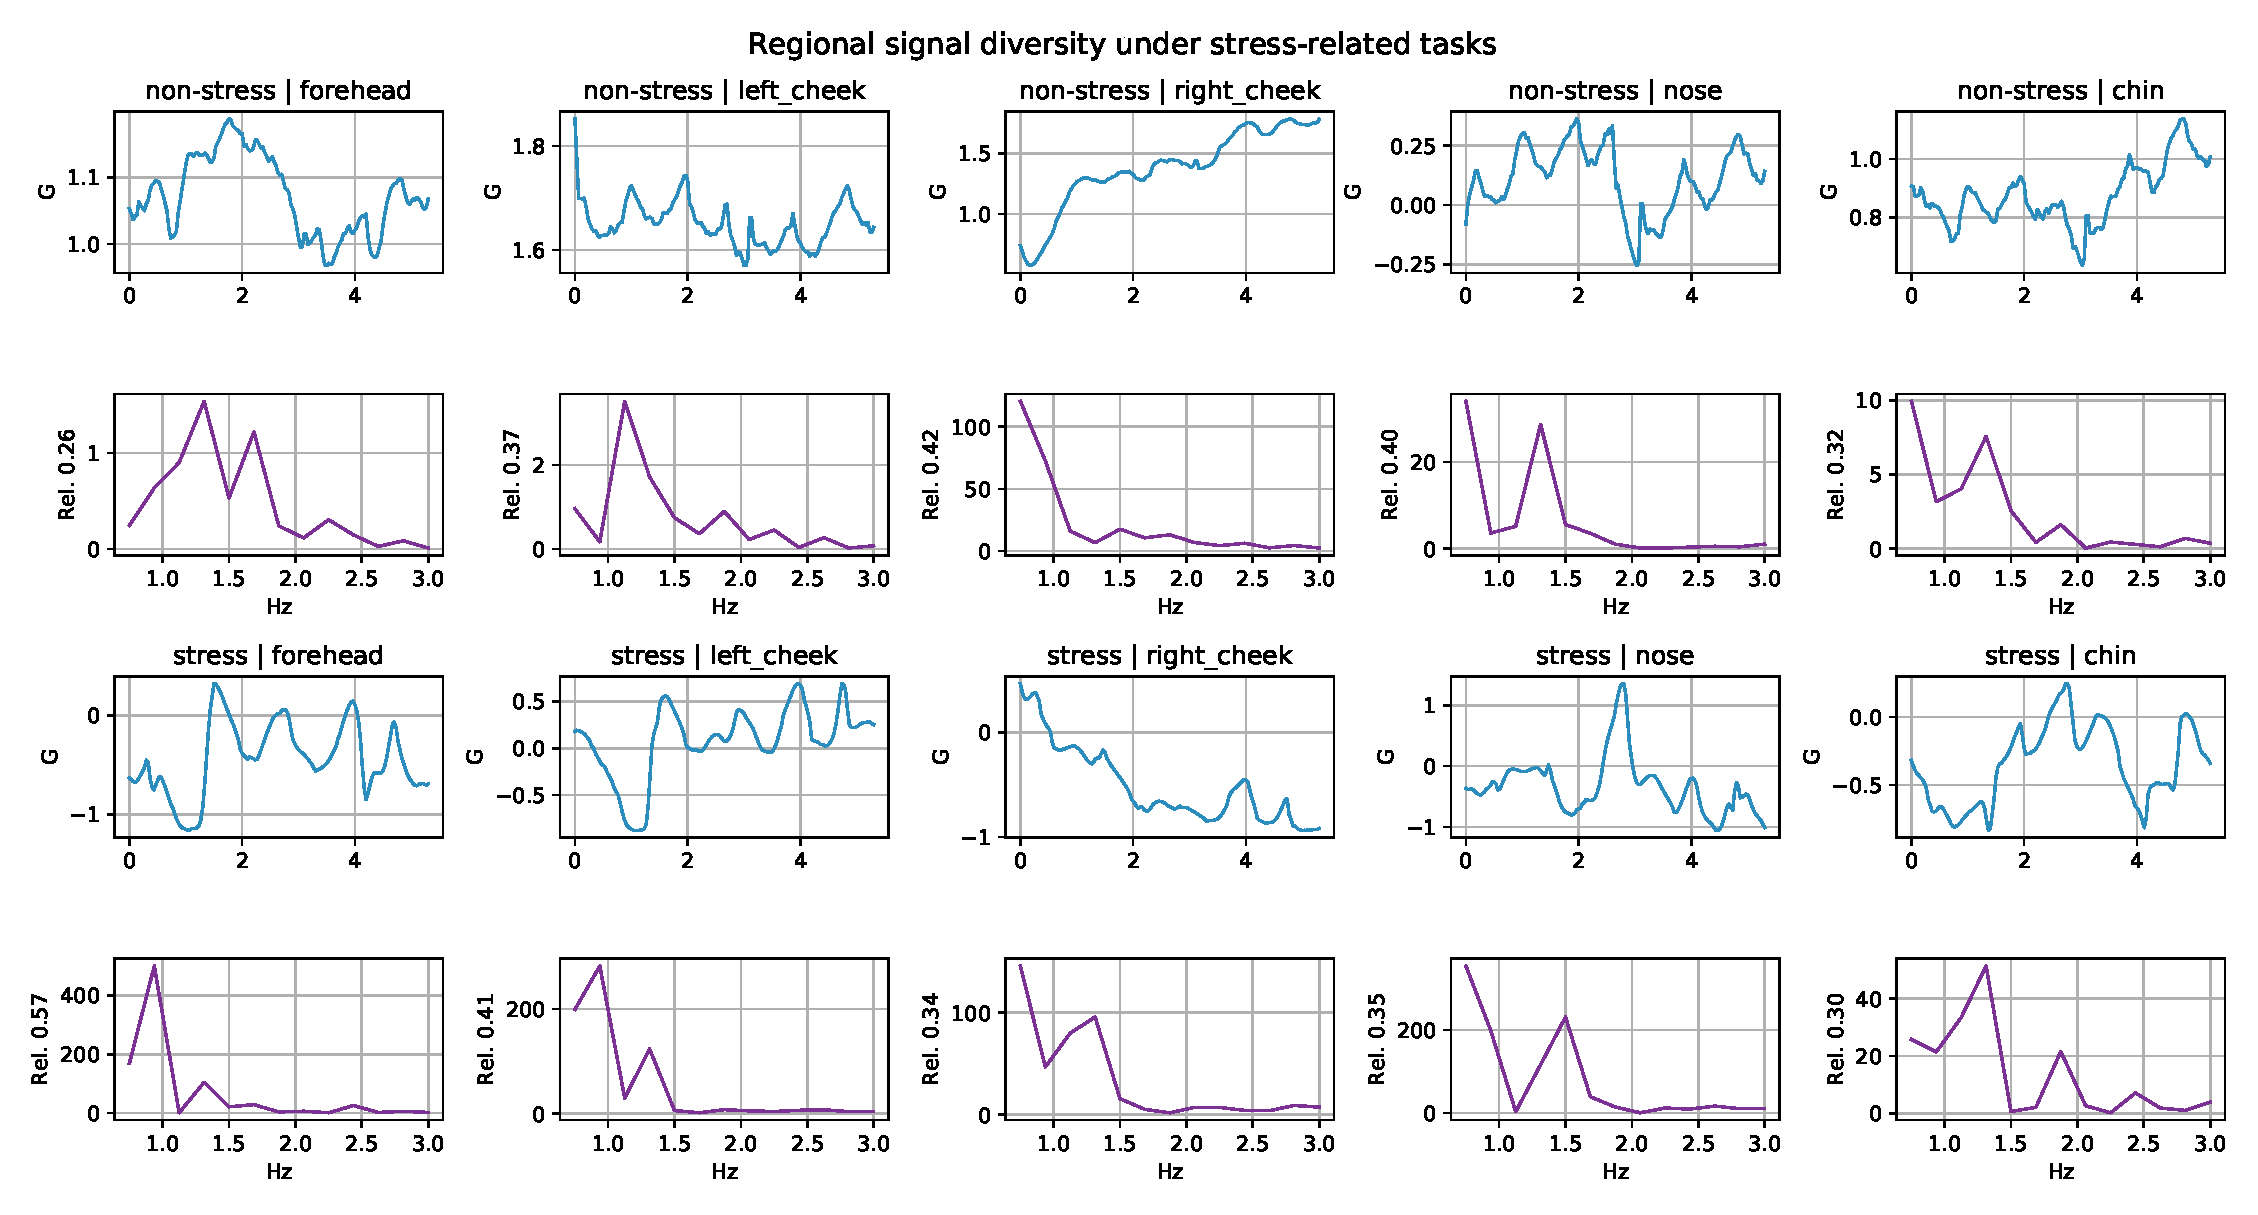
\includegraphics[width=0.92\textwidth,height=0.18\textheight,keepaspectratio]{f3.eps}%
}{%
\figplaceholder{Fig. 3 Quantitative Evaluation}{ROC curves for RT-MRCPNet and representative baselines, together with the RT-MRCPNet confusion matrix under the subject-independent test protocol.}%
}
\caption{Quantitative visualization of the subject-independent evaluation. The receiver operating characteristic curves compare the proposed method with representative baselines, and the confusion matrix summarizes the error distribution of RT-MRCPNet. This view complements Table~\ref{tab:main_results} by making the ranking and error pattern easier to inspect.}
\label{fig:quantitative_visualization}
\end{figure}

Table~\ref{tab:main_results} and Fig.~\ref{fig:quantitative_visualization} show that RT-MRCPNet performs best among all compared RGB-sequence, rPPG-feature, and lightweight video baselines. The left- and right-cheek single-region models are stronger than the nose- and chin-only models, indicating that regional signal quality is uneven. RT-MRCPNet further improves over fixed multi-region fusion, which suggests that adaptive temporal and regional weighting is useful beyond simply using more ROIs.

\subsection{Ablation Study}

The ablation study further decomposes the proposed model. It uses the same protocol as Table~\ref{tab:main_results}. In contrast to the controlled comparison, which changes the input representation or fusion strategy, this section removes individual attention modules from RT-MRCPNet to test whether each component contributes to the final prediction.

\begin{table}
\caption{Ablation study of the proposed method. ACC denotes accuracy, AUC denotes area under the receiver operating characteristic curve, and RT-MRCPNet denotes Region-Temporal Attention Multi-Region Color Pulse Network. All metrics are reported in percentage (\%).}
\label{tab:ablation}
\centering
\begin{tabular}{lccc}
\toprule
Variant & ACC & F1 & AUC \\
\midrule
Without attention & 83.62 & 83.04 & 86.44 \\
Temporal attention only & 86.15 & 85.52 & 88.90 \\
Region attention only & 85.34 & 84.71 & 88.22 \\
Full RT-MRCPNet & \textbf{88.42} & \textbf{88.15} & \textbf{91.54} \\
\bottomrule
\end{tabular}
\end{table}

The ablation results in Table~\ref{tab:ablation} confirm the complementarity of the two attention stages. Removing both attention modules reduces the model to fixed multi-region fusion. Adding temporal attention or region attention alone improves performance, and using both gives the best result.

\begin{figure}
\centering
\IfFileExists{f4.eps}{%
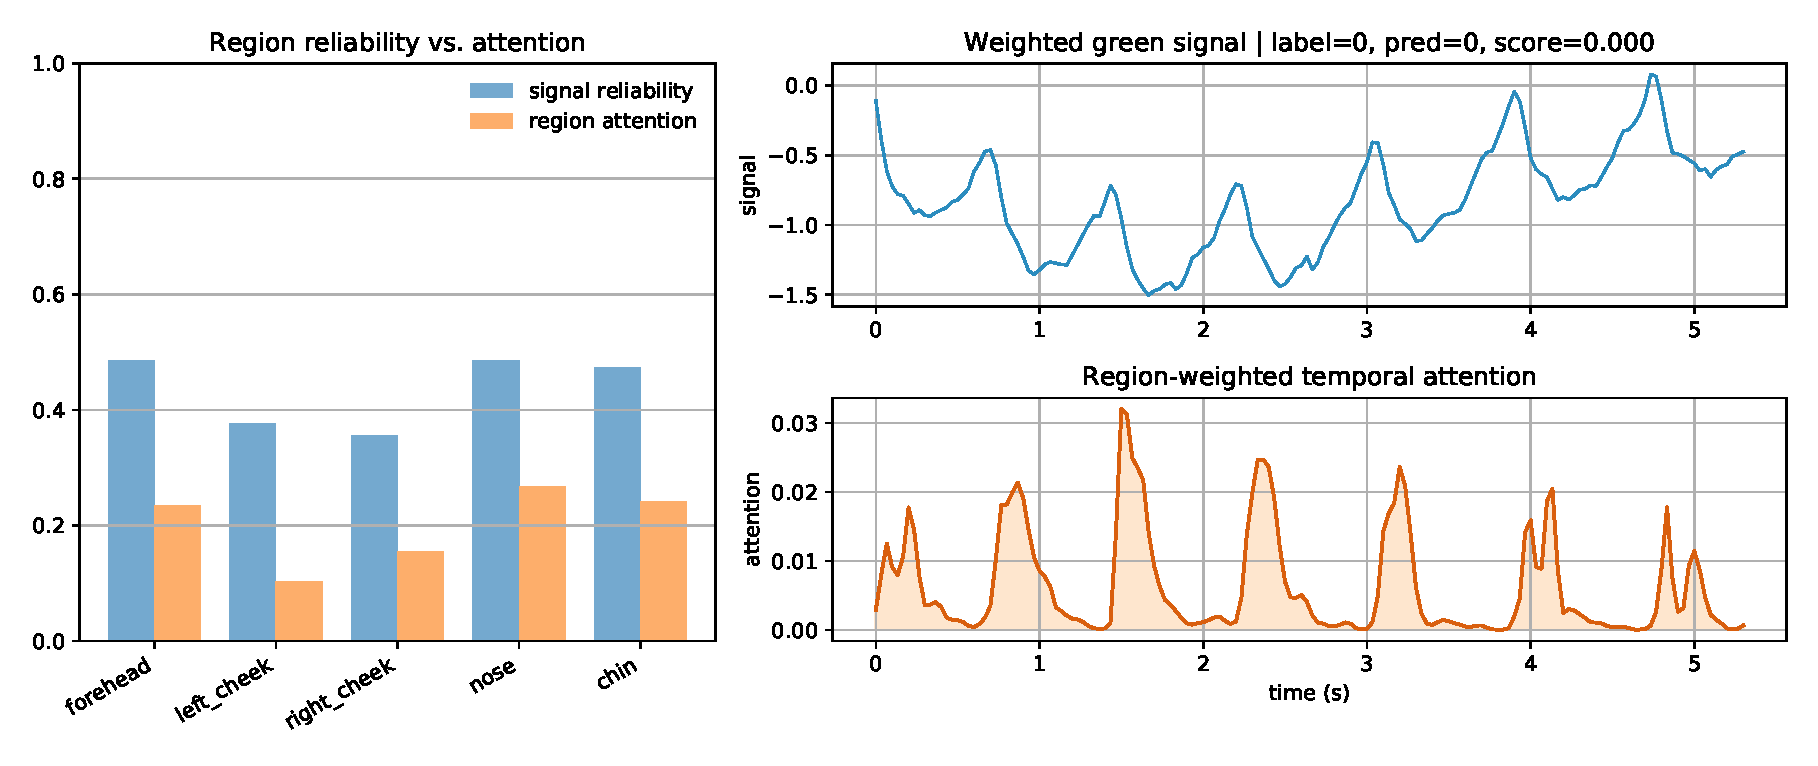
\includegraphics[width=0.92\textwidth,height=0.18\textheight,keepaspectratio]{f4.eps}%
}{%
\figplaceholder{Fig. 4 Attention Visualization}{ROI attention weights over the five facial regions and temporal attention curves for representative stress and non-stress clips.}%
}
\caption{Attention-based qualitative visualization. Region attention over the five facial ROIs and temporal attention curves for representative stress and non-stress clips indicate whether the model emphasizes physiologically plausible regions and suppresses unstable temporal segments.}
\label{fig:attention_visualization}
\end{figure}

\subsection{Complexity Analysis}

RT-MRCPNet uses compact regional RGB sequences instead of full facial frames. Its input size is $K \times T \times 3$, which is much smaller than $T \times H \times W \times 3$ for full-frame video models. Table~\ref{tab:complexity} reports the parameter count, floating-point operations (FLOPs), and inference time of representative baselines.

\begin{table}
\caption{Model complexity comparison. RGB denotes red-green-blue, 3D denotes three-dimensional, CNN denotes convolutional neural network, FLOPs denotes floating-point operations, and RT-MRCPNet denotes Region-Temporal Attention Multi-Region Color Pulse Network.}
\label{tab:complexity}
\centering
\begin{tabular}{lccc}
\toprule
Method & Parameters & FLOPs & Inference Time \\
\midrule
Full-frame convolutional recurrent network & 12.54M & 15.20G & 35.42 ms \\
Full-frame 3D convolutional neural network & 33.25M & 38.64G & 42.15 ms \\
Full-face RGB temporal network & 0.82M & 0.05G & 1.25 ms \\
RT-MRCPNet & 0.94M & 0.25G & 2.38 ms \\
\bottomrule
\end{tabular}
\end{table}

\section{Conclusion}

This paper presents RT-MRCPNet, a lightweight region-temporal attention network for contactless stress recognition from facial videos. The method converts facial clips into compact multi-region RGB temporal sequences, models local color dynamics with a shared temporal encoder, and adaptively aggregates information through temporal and region attention. Under a subject-independent protocol, RT-MRCPNet achieves 88.42\% ACC, 88.15\% F1-score, and 91.54\% AUC, outperforming the compared RGB sequence, hand-crafted rPPG feature, and lightweight video baselines. The ablation and complexity analyses show that temporal and region attention bring complementary gains while keeping the model efficient. The current method still uses fixed rectangular ROIs and binary task labels; future work will explore landmark- or mesh-based region definitions, finer-grained stress annotations, and multimodal fusion with audio, gaze, or contact physiological signals.

\begingroup
\let\small\footnotesize
\bibliographystyle{splncs04}
\bibliography{references}
\endgroup

\end{document}
